\begin{frame}
    \frametitle{Die Bourne-Again-Shell}
    
\includegraphics[height=1.2cm]{res/bash.png}
    \begin{itemize}
        \item Veröffentlicht \textbf{1989} (vor 28 Jahren)
        \item Nachfolger der Bourne-Shell (daher der Name)
        \item Kurz \textbf{bash}
        \item Kombiniert Skript-Syntax der \textbf{sh} mit den interaktive Funktionen der \textbf{csh}
        \item Heute der Standard unter \textbf{Linux} und \textbf{macOS}
    \end{itemize}
\end{frame}

\begin{frame}
    \frametitle{BusyBox}
    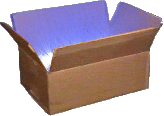
\includegraphics[height=1.2cm]{res/busybox.png}
    \begin{itemize}
        \item Mehr als eine Shell
        \item Viele sonst selbständige Tools in einer \textbf{einzigen Datei}
        \item Dadurch weniger Overhead
        \item Beliebt im Embedded-Bereich und z.B. als Notfall-Shell
    \end{itemize}
\end{frame}

\begin{frame}
    \frametitle{Debian-Almquist-Shell}
    \begin{itemize}
        \item Verbesserung der \textbf{Almquist-Shell} (von Kenneth Almquist) für die Debian-Linux-Distribution
        \item Leichtgewichtig
        \item In Debian und Ubuntu daher Standard für Skript-Ausführung
        \item Im Embedded-Bereich beliebt
    \end{itemize}
\end{frame}

\begin{frame}
    \frametitle{PowerShell}
    
\includegraphics[height=1.2cm]{res/powershell.png}
    \begin{itemize}
        \item \textbf{2006} entwickelt von Microsoft
        \item Ersatz für die alte und leistungsschwache cmd.exe
        \item Open-Source und auch unter Linux nutzbar
        \item Funktionsreiche Skriptsprache basierend auf .NET
    \end{itemize}
\end{frame}
